%------------------------------------------------------------------------------
% Template file for the submission of papers to IUCr journals in LaTeX2e
% using the iucr document class
% Copyright 1999-2013 International Union of Crystallography
% Version 1.6 (28 March 2013)
%------------------------------------------------------------------------------

\documentclass[a4paper,12pt,oneside]{article}              % DO NOT DELETE THIS LINE

     %-------------------------------------------------------------------------
     % Information about journal to which submitted
     %-------------------------------------------------------------------------
%     \journalcode{J}              % Indicate the journal to which submitted
                                  %   A - Acta Crystallographica Section A
                                  %   B - Acta Crystallographica Section B
                                  %   C - Acta Crystallographica Section C
                                  %   D - Acta Crystallographica Section D
                                  %   E - Acta Crystallographica Section E
                                  %   F - Acta Crystallographica Section F
                                  %   J - Journal of Applied Crystallography
                                  %   M - IUCrJ
                                  %   S - Journal of Synchrotron Radiation
\usepackage{natbib}
\usepackage{graphicx}
\usepackage[T1]{fontenc}
\usepackage[utf8]{inputenc}
\usepackage{amsmath}
\usepackage{fancyhdr}
\usepackage{lineno}

\newcommand{\citeasnoun}{\citet}
\newcommand{\volbf}{\textbf}
\linespread{2}

\pagestyle{fancy}
\fancyhf{}
\fancyhead[LE,RO]{2022-04-06}
\fancyhead[RE,LO]{Jérôme Kieffer}
%\fancyfoot[CE,CO]{\leftmark}
\fancyfoot[CE,CO]{\thepage}


\begin{document}                  % DO NOT DELETE THIS LINE
\linenumbers

     %-------------------------------------------------------------------------
     % The introductory (header) part of the paper
     %-------------------------------------------------------------------------

     % The title of the paper. Use \shorttitle to indicate an abbreviated title
     % for use in running heads (you will need to uncomment it).

\title{Application of signal separation to diffraction image compression and serial crystallography}
%\shorttitle{Short Title}

     % Authors' names and addresses. Use \cauthor for the main (contact) author.
     % Use \author for all other authors. Use \aff for authors' affiliations.
     % Use lower-case letters in square brackets to link authors to their
     % affiliations; if there is only one affiliation address, remove the [a].

%\cauthor[a]{Jérôme}{Kieffer}{jerome.kieffer@esrf.fr}{}
%\author[a]{Nicolas}{Coquelle}
%\author[a]{Samuel}{Debionne}
%\author[b]{Shibom}{Basu}
%\author[a]{Alejandro}{Homs}
%\author[a]{Gianluca}{Santoni}
%\author[a]{Götz}{Andrew}
%\author[a]{Daniele}{De Sanctis}

%\aff[a]{European Synchrotron Radiation Facility;71, avenue des Martyrs;CS 40220;38043 Grenoble Cedex 9 \country{France}}
%\aff[b]{EMBL Grenoble; 71 avenue des Martyrs; CS 90181; 38042 Grenoble Cedex 9; \country{France}}

     % Use \shortauthor to indicate an abbreviated author list for use in
     % running heads (you will need to uncomment it).

%\shortauthor{Soape, Author and Doe}

     % Use \vita if required to give biographical details (for authors of
     % invited review papers only). Uncomment it.

%\vita{Author's biography}

     % Keywords (required for Journal of Synchrotron Radiation only)
     % Use the \keyword macro for each word or phrase, e.g. 
     % \keyword{X-ray diffraction}\keyword{muscle}

%\keyword{keyword}

     % PDB and NDB reference codes for structures referenced in the article and
     % deposited with the Protein Data Bank and Nucleic Acids Database (Acta
     % Crystallographica Section D). Repeat for each separate structure e.g
     % \PDBref[dethiobiotin synthetase]{1byi} \NDBref[d(G$_4$CGC$_4$)]{ad0002}

%\PDBref[optional name]{refcode}
%\NDBref[optional name]{refcode}

\maketitle                        % DO NOT DELETE THIS LINE

%\begin{synopsis}
%Precise background assessment and application to single crystal image compression and serial crystallography data reprocessing. 
%\end{synopsis}

%\begin{abstract}
%Abstract goes here.
%\end{abstract}


     %-------------------------------------------------------------------------
     % The main body of the paper
     %-------------------------------------------------------------------------
     % Now enter the text of the document in multiple \section's, \subsection's
     % and \subsubsection's as required.

\section{Introduction}
\subsection{Serial crystallography on synchrotron sources (SSX)}
%not sure we need subsections here
Serial crystallography is a relatively new technique in structural biology. 
It is composed of several techniques where multiple crystals (hundreds or thousands) are exposed in a serial way to the X-ray beam to collect a complete dataset. 
This is in contrast with traditional rotational crystallography, where a complete dataset is collected from a single crystal rotated around one (or several) axis. 
The serial approach is particularly useful to try to overcome the limitations of radiation damage, in particular in very small crystals.
The technique was first developed for X-ray free electron lasers (XFEL) \cite{Chapman2011}
but recently also adapted to be performed at synchrotron light sources.
Macromolecular crystallography beamlines (MX) have been extremely specialized towards rotational data collection and are thus not well addapted to SSX.
The higher flux requirement for SSX make it a clear candidate to be performed at 4\textsuperscript{th} generation synchrotron sources, like the new ESRF-EBS update \cite{EBS}.
The Synchrotron serial crystallography beamline (ID29 at the ESRF) has been built to have a dedicated environment to perform SSX experiments with a high flux (thanks to multi-layer optics), a high-speed chopper, several sample delivery methods and a fast detector.
\subsection{Jungfrau4M detector}
Unlike photon counting detectors like the Eiger detector \cite{Eiger}, the Jungfrau (developed at PSI) is an integrating detector which is not limited by the count rate, even under very intense flux as expected when recording Bragg-peaks \cite{jungfrau2016}.
To cope with this very large number of photons, every single pixel implements an automatic gain switching mechanism (3 levels) which offers a precision on the order of a fraction of a keV on the higher gain mode, a precision of the order one a photon in the intermediate level and the ability to cope with thousands of photons per millisecond in the lower gain mode.
Since the Jungfrau is an integrating detector, every pixel has has three dark-current values, called pedestal and three gain values (one for each gain level). 
This large number of parameters per pixel combined with the gain-compression makes the preprocessing of raw signal challenging: the signal from a single pixel, initially stored on 16 bits of data, needs to be represented using 32 bits (as floating point or integer value), doubling the storage size \cite{jungfrau_PSI}.
The ID29 beamline features a Jungfrau 4M detector, operating at 1kHz, pace imposed by a chopper and synchronized with the photon bunches from the ESRF.
The data analysis and storage are thus anticipated to be extremely challenging. 
\subsection{Requirements for online data processing}
%again, this is not great, as it is not the text below. 
Efficient processing of raw images is vital for SSX.
Multiple challenges are present, in particular partiality and low completeness of data collected for each individual crystal.
To this reason, careful and precise location of Bragg peaks is vital.

\section{Algorithm for the separation of amorphous background from Bragg peaks}
\subsection{Background scattering}

The simplest implementation of Bragg peaks separation is to consider that the background originates from scattering from amorphous material or from an isotropic powder, both giving isotropic signal ideally presenting only smooth variations.
For this, the raw signal has to be corrected from dark noise and any systematic anisotropic effects like polarization corrections.
Unlike X-FEL, synchrotron X-ray beam show little bunch to bunch variability and with the beam being well characterized, those anisotropic correction can be easily taken into account.

The initial implementation in pyFAI \cite{pdj2013} used to rely on a 2D polar transform followed by a median filter in the azimuthal dimension 
to separate amorphous scattering from single crystal scattering.
Despite this method has been successfully used for large dataset analysis \cite{brocades}, it presents several major drawbacks:
\begin{itemize}
\item The 2D averaging mixes the signal of several pixels and blurs the signal. 
\item Pixel-splitting is needed to leverage the Moiré effect in the 2D averaging, but this increases further the blurring. 
\item The 1D curve obtained after the application of the median filter shows sharp jumps from one azimuthal bin to its neighbour.
\item Median filter is computationally heavy since it requires to sort out every azimuthal bin.
\end{itemize}

The coming sections present an efficient way to perform the azimuthal averaging (including the associated variance propagation),  its application to the statistical analysis and extraction of background from a diffraction image. 

\subsection{Efficient azimuthal averaging and uncertainties evaluation}

\subsubsection{Preprocessing:}
The first step of the analysis consists in applying a pixel-wise correction for dark current and several normalization corrections \cite{pyfai_2020}:
\begin{equation}
\label{norm}
I_{cor} = \frac{signal}{norm}  = \frac{I_{raw} - I_{dark}}{F \cdot
\Omega \cdot P \cdot A \cdot I_0} 
\end{equation}
In  equation \ref{norm}, the numerator (refereed as $signal$ hereafter) is the subtraction of the dark current $I_{dark}$ from the the detector's raw signal $I_{raw}$.
The denominator (hereafter $norm$) is a normalization factor composed of the product of  $F$:  a factor accounting for the flat-field correction, $\Omega$: the solid angle subtended by a given pixel, $P$: the polarisation correction term and $A$: the detector's apparent efficiency due to the incidence angle of the photon on the detector plane (for integrating detectors, high energy photons with larger incidence angle see larger sensor thickness, and thus have higher detection probability).
Intensity is also normalized by the incoming flux $I_0$, but since it is independent from the pixel position this correction has no influence.

\subsubsection{Azimuthal averaging:} 

Historically, the azimuthal averaging was implemented using histograms. 
Since the geometry of the experimental setup is fixed during the acquisition, a look-up table listing all pixels contributing to each  azimuthal-bin can be built and used to speed-up calculations \cite{pyFAI_gpu}.
The azimuthal transformation being a linear transformation, it can be implemented as a matrix multiplication, with a sparse-matrix representing the transformation and a dense vector which is simply the flattened view of the diffraction image. 
The compressed sparse row (CSR) matrix representation is preferred for its efficiency in performing dot products with dense vectors \cite{SpMV}.
The coefficients $c_{i,r}$ of the matrix are the fraction of area of a pixel $i$ falling into the radial bin $r$.
In the case where pixel splitting is deactivated those coefficients  ($c_{i,r}$) are always one (and zero elsewhere) since each pixel contribute to a single bin.
The sparse matrix multiplication can be used to sum efficiently values for all pixels belonging to the same bin.
The summed signal divided by the summed normalization provides the weight-averaged intensity over all pixels falling in the bin at the distance $r$ from the center, as formalized in equation \ref{avg}: 
\begin{equation}
\label{avg}
<I>_{r} = \frac{\sum\limits_{i \in bin_r} c_{i,r} \cdot signal_i}
                        {\sum\limits_{i \in bin_r} c_{i,r} \cdot norm_i} 
\end{equation}  

\subsubsection{Uncertainty evaluation from Poisson law:}
Photon counting detectors, like Eiger detectors, suffer from hardly any error beside the counting uncertainty which is often referred as Poisson statistics.
This statistical law states that the variance for a pixel is the number of events counted.
Other sources of noise, like the dark current noise in the case of an integrating detector,  superimpose quadratically to the Poisson noise for integrating detectors, as presented in equation \ref{poisson}:     
\begin{equation}
\label{poisson}
var_I = (\sigma_I)^{2} = I_{raw} + (\sigma_{dark})^{2}  
\end{equation}

During the azimuthal integration, the coefficient of the sparse matrix needs to be squared at the numerator when propagating the variance (equation \ref{varianceP}) to have uncertainties $\sigma$ proportional to the fraction of the pixel considered.
\begin{equation}
\label{varianceP}
(\sigma_{r}(I))^2 = \frac{\sum\limits_{i \in bin_r} c_{i,r}^2 \cdot \sigma_i^2}
                  {\sum\limits_{i \in bin_r} c_{i,r} \cdot norm_i} 
\end{equation}
One should distinguish the \textit{uncertainty of the mean} (sometimes referred are standard error of the mean or $sem$), 
which describes the precision with which the mean is known (and described in \citeasnoun{pyfai_2020}),
from the \textit{uncertainty of the pixel value} (often referred as standard deviation, $std$). 
Those two value differ only by square root of the number of measurements in the case of an arithmetic mean: $sem = std/\sqrt{N}$ with $N$ the number of pixel contributing to the bin.
When considering the weighted average, the previous formula becomes:
\begin{equation}
\label{sem}
sem_r = std_r \frac{\sqrt{\sum\limits_{i \in bin_r} c_{i,r}^2 \cdot norm_i^2}}{\sum\limits_{i \in bin_r} c_{i,r} \cdot norm_i}
\end{equation}
Thus, the more data point are collected, the more precisely the mean value is known.
Since this document focuses on the uncertainties of pixel values, the \textit{standard deviation} will systematically be used in this document.  

\subsubsection{Uncertainty evaluation from the variance in a bin:}

Unlike photon counting detectors, most detectors are not following the Poisson law and the establishment of a formula $\sigma^2 = f(I)$ is not simple, if possible at all. 
In the case of the Jungfrau detector considered for the ESRF-ID29 beamline, this integrating detector has a complex gain switching mechanism \cite{jungfrau_PSI} which makes this equation complicated.
A generic approach is proposed here to measure the variance in every single bin.

When considering the diffraction of an isotropic compound (liquid, amorphous or perfect powder), all pixels falling into the same radial bin should see the same flux of photons and the deviation to their intensities could be used to estimate the uncertainty. 
This approach is of course limited when considering Bragg-peaks, but it provides an upper bound for the uncertainty.
Variance (and standard deviation) are usually obtained in a two steps procedure: one pass to calculate the average value (equation \ref{avg}) and a second to calculate the deviation to the average (equation \ref{varA}). 
This double pass approach can be implemented using sparse matrix multiplication. 
It requires itwice the access to each pixel, and extra storage space, but it is numerically more robust (less probe to numerical error accumulation).
\begin{equation}
\label{varA}
    (\sigma_{r}(I))^2 = \frac {\sum\limits_{i \in bin_r} c_{i,r} \cdot norm_i \cdot (\frac{signal_i}{norm_i}-<I>_r)^2}
                              {\sum\limits_{i \in bin_r} c_{i,r} \cdot norm_i}
\end{equation}
and:
\begin{equation}
\label{varB}
(\sigma_{r}(<I>))^2 = \frac{\sum\limits_{i \in bin_r} c_{i,r}^2 \cdot norm_i^2 \cdot (\frac{signal_i}{norm_i}-<I>_r)^2}
                         {(\sum\limits_{i \in bin_r} c_{i,r} \cdot norm_i)^2}  
\end{equation}


Single pass implementations of variance calculation are faster since they access pixels only once and offer the ability to perform parallel reductions \cite{Blelloch}, i.e. work with blocks of pixels .
\citeasnoun{variance2018} presents a complete review, from which we adapt to the formalism of crystallography some key equations.
For example the weight for a pixel is $\omega_i = c_i \cdot norm_i$.
If $P$ is a partition of the ensemble of pixels falling into a given azimuthal bin, let $\Omega_{P}$, $V_{P}$ and $VV_{P}$  
be the sum of weights (Eq \ref{omega}), the weighted sum of $V$ (Eq \ref{Vp}) and the weighted sum of deviation squared (Eq \ref{VVp}) over the partition $P$: 
\begin{equation}
\label{omega}
\Omega_{P} = \sum\limits_{i \in P} \omega_i = \sum\limits_{i \in P} c_i \cdot norm_i 
\end{equation}
\begin{equation}
\label{Vp}
V_{P} = \sum\limits_{i \in P} \omega_i \cdot v_i =  \sum\limits_{i \in P} c_i \cdot signal_i
\end{equation}
\begin{equation}
\label{VVp}
VV_{p} = \sum\limits_{i \in P} \omega_i \cdot (v_i - V_{P}/\Omega_{P})^2 
\end{equation}

The average and the variance are then expressed as:
\begin{equation}
<I>_P = \frac{V_{P}}{\Omega_{P}} =  \frac{\sum\limits_{i \in P} c_i \cdot signal_i}
                        {\sum\limits_{i \in P} c_i \cdot norm_i} 
\end{equation}

\begin{equation}
(\sigma_P(I))^2 = \frac{VV_{P}}{\Omega_{P}}
\end{equation}

Performing the union of two partitions $A$ and $B$ allows the parallel reduction, which is especially efficient on GPU:
\begin{equation}
\Omega_{A \cup B} =  \Omega_{A} + \Omega_{B} 
\end{equation}

\begin{equation}
V_{A \cup B} =  V_{A} + V_{B} 
\end{equation}
  
\begin{equation}
VV_{A \cup B} =  VV_{A} + VV_{B} +  \frac{(\Omega_{A} \cdot V_{B} - \Omega_{B}\cdot V_{A})^2}{V_{A \cup B} \cdot  V_{A} \cdot V_{B}}
\end{equation}
  
The numerical stability issue is addressed by using double-precision arithmetic when implemented on CPU and double-word arithmetic when running on GPU \cite{double_word}.

\subsection{Histogram intensity }

The figure \ref{fig1}a presents the diffraction from a single crystal of insulin and several curves obtained from azimuthal integration: 
\ref{fig1}b is the azimuthally integrated signal (blue curve). Bragg peaks are seen as spikes on top of a smooth background.
The plot \ref{fig1}c presents the uncertainties measured according to the Poisson law (orange curve, valid since the Pilatus is a photon counting detector) 
or the deviation in the ring (blue curve), much larger value since Bragg peaks contribute a lot to the deviation despite they represent few pixels.
This highlights the sensitivity of the mean/std to ouliers.
In the plot \ref{fig1}d are presented histogram of pixel intensity for pixels laying at 80mm and 160mm from the beam center. 
Each of those histograms is composed of a bell-shaped distribution, centered on the average value with negative outliers tagged with the pixel value -1 (this is specific to the Pilatus detector), and few positive outliers which are usually Bragg peaks.   
Those histograms in figure \ref{fig1}d have been fitted with a Gaussian curve and both the center ($\mu$) and the width ($\sigma$) of the curve match 
roughly with the average (in \ref{fig1}b) and uncertainties (in \ref{fig1}c).  
\begin{figure}
\label{fig1}
\begin{center}
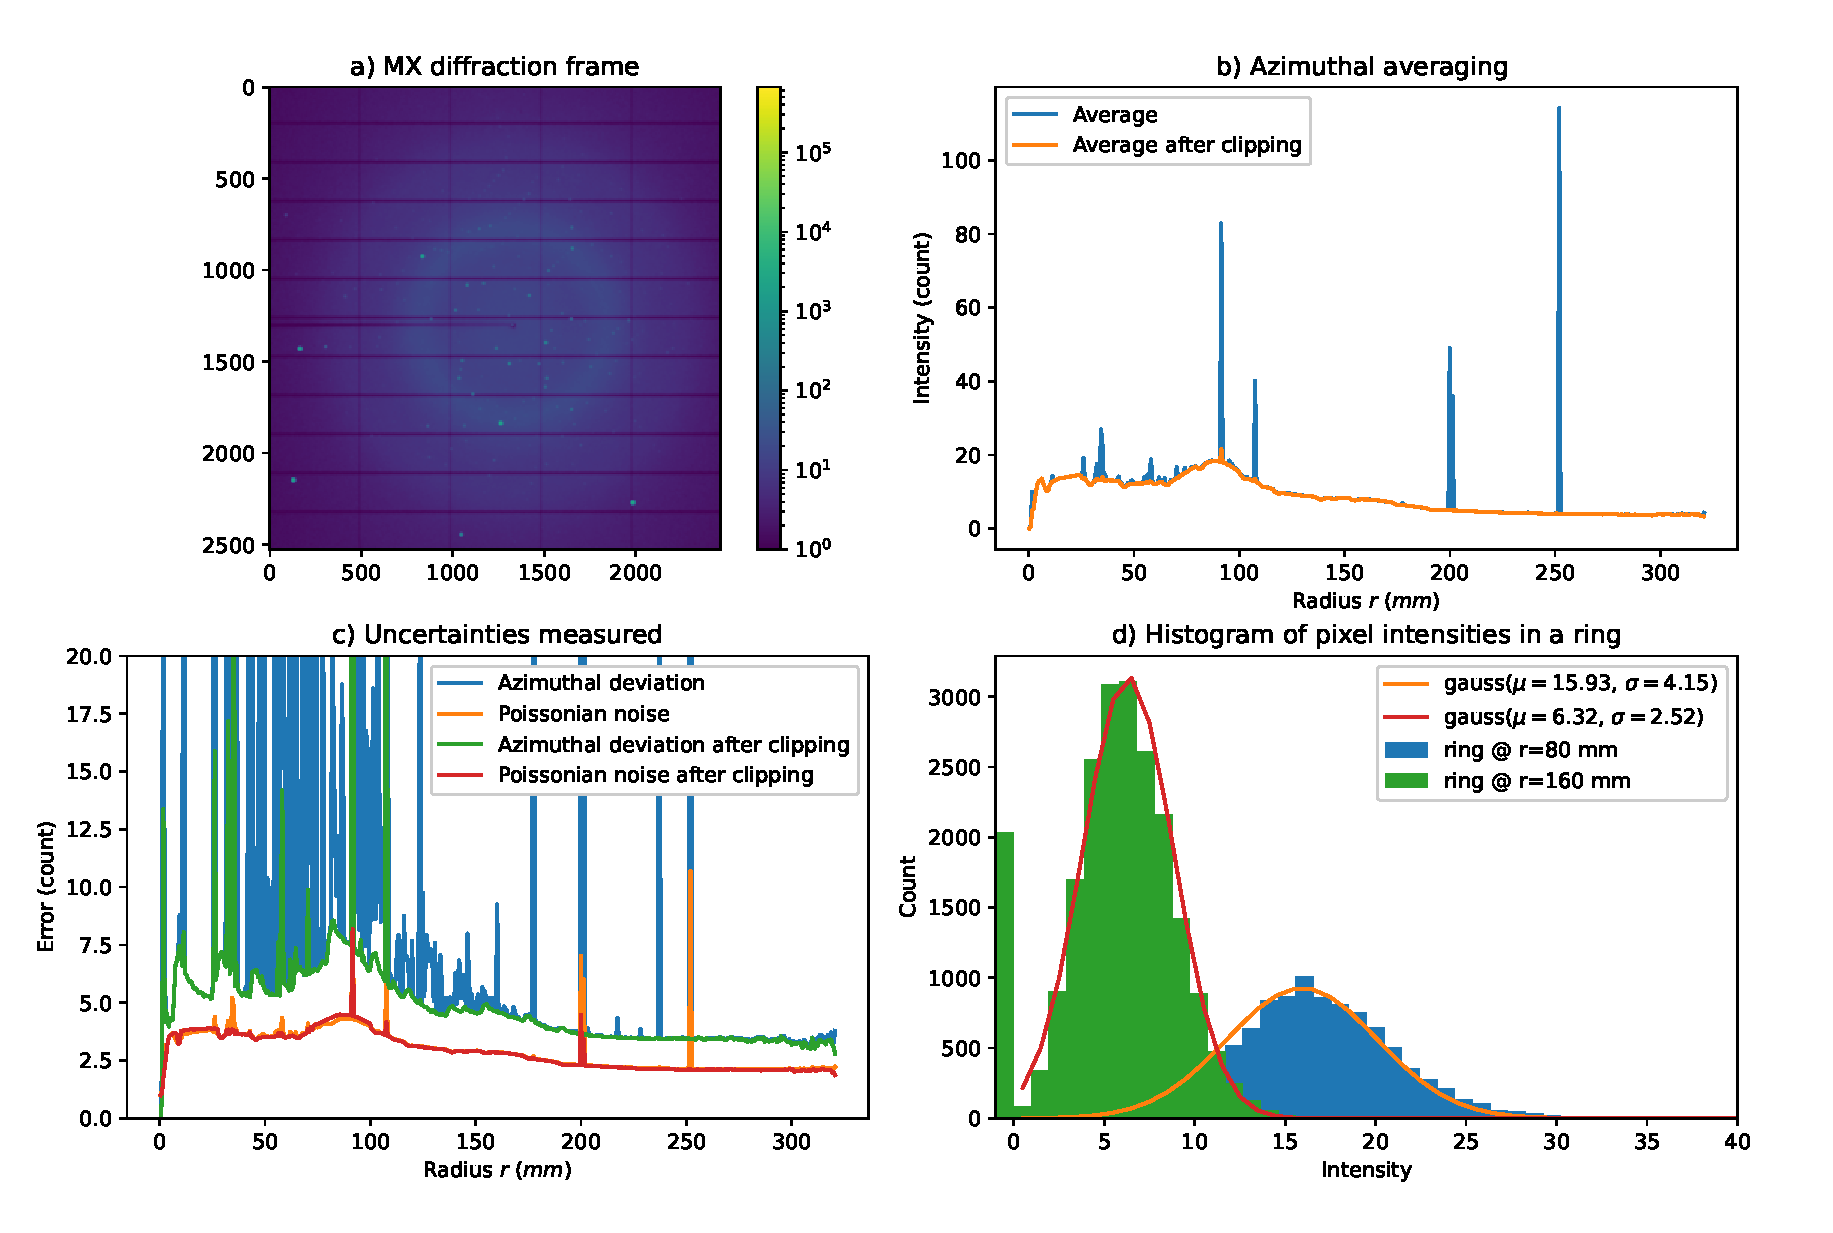
\includegraphics[width=14cm]{fig1}
\caption{Single crystal diffraction frame obtained from insulin with a Pilatus6M (a) (part of Dectris's reference dataset) with the azimuthally averaged signal (b), 
before and after clipping data. Uncertainties are presented in (c) when calculated assuming a Poissonian error model or when measuring the deviation within all pixels in a ring.
Subplot (d) presents the histogram of intensities for two rings at r=80mm and r=160mm from beam center with the distribution fitted as Gaussians.}
\end{center}
\end{figure}

The core idea of the algorithm for background extraction is to model the distribution of background pixels. Unlike Bayesian statistics \cite{Sivia2006} where the cost function is usually tuned to weight less outlier, here, those outliers are simply flagged and discarded.
Positive outliers can reasonably be assigned to Bragg peaks and negative outliers to shadows or defective pixels. 
The distribution is recalculated  after discarding pixels for which intensity differ from the average value by more than $n$ times the standard deviation (Eq\ref{clip}) which has the effect of re-centering the distribution and enforcing a normal distribution of the remaining values:
\begin{equation}
\label{clip}
|I - <I>| > n \cdot \sigma(I)
\end{equation}
The orange plot in figure \ref{fig1}b presents the average after having discarded those outliers, and the orange and green curve of figure \ref{fig1}c are the uncertainties calculated after this clipping. 
After clipping, the average and uncertainties curves have lost most of their spikes, which means that Bragg peaks and shadowed pixel were discarded.
 
\subsection{Sigma-clipping}
The \textit{sigma-clipping} algorithm consists in applying the outlier rejection previously described several times, in order to enforce the background distribution to follow a normal law.
There are two parameters to this algorithm: the number of iterations and the rejection cut-off.
%I merged number of iterations and sigma clipping  as closely connected.
Despite the execution time is proportional to the number of iteration of sigma-clipping, iterations should continue until no more outliers are found and the 
background distribution actually matches a normal distribution (Gaussian). 
Since the loop exits as soon as no more outliers were discarded at the clipping step, having an arbitrary large number of iteration is not really an issue for the execution time and the number of actual iteration is usually few (3 is commonly observed).       

\subsubsection{Clipping threshold}
can be automatically calculated based on a variation on Chauvenet's criterion \cite{chauvenet} where one would accept to discard only a single pixel in a ring with a signal already following a normal law. 
Thus, the threshold value is adapted to the $size$ of the distribution, i.e. the number of pixels in each ring (Eq\ref{chauvenet}), which can reach several thousands and shrinks with iterations.
Typically the numerical value for this cut-off varies from 2 to 4.   
\begin{equation}
\label{chauvenet}
SNR_{chauvenet} =  \sqrt{2 log(\frac{size}{\sqrt{2 \pi}})}
\end{equation}
% could be interesting to show Threshold vs cycle for the example above (if relecant)

\section{Application to single crystal diffraction image compression}
%I explicit here MAcromolecular as we are talking about id29. Remove is superfluous.
Diffraction images from a single macromolecular crystal exhibit usually an isotropic background on top of which Bragg peaks appear.
The sigma-clipping algorithm can be used to select the background level and more importantly the associated uncertainty.

This lossy compression algorithm consists in picking (and storing) pixels which intensity is above the average background value ($\mu$) plus $n$ standard deviation ($\sigma$). 
This cut-off value $n$ controls the amount of data to store and provides also a hint for the compression ratio achievable, assuming a normal distribution has been enforced at the sigma-clipping stage: 16\% of the pixel are to be recorded with $n=1$;  2.3\% for $n=2$ and only 0.13\% for $n=3$ as depicted in figure \ref{distribution}.
\begin{figure}
\label{distribution}
\begin{center}
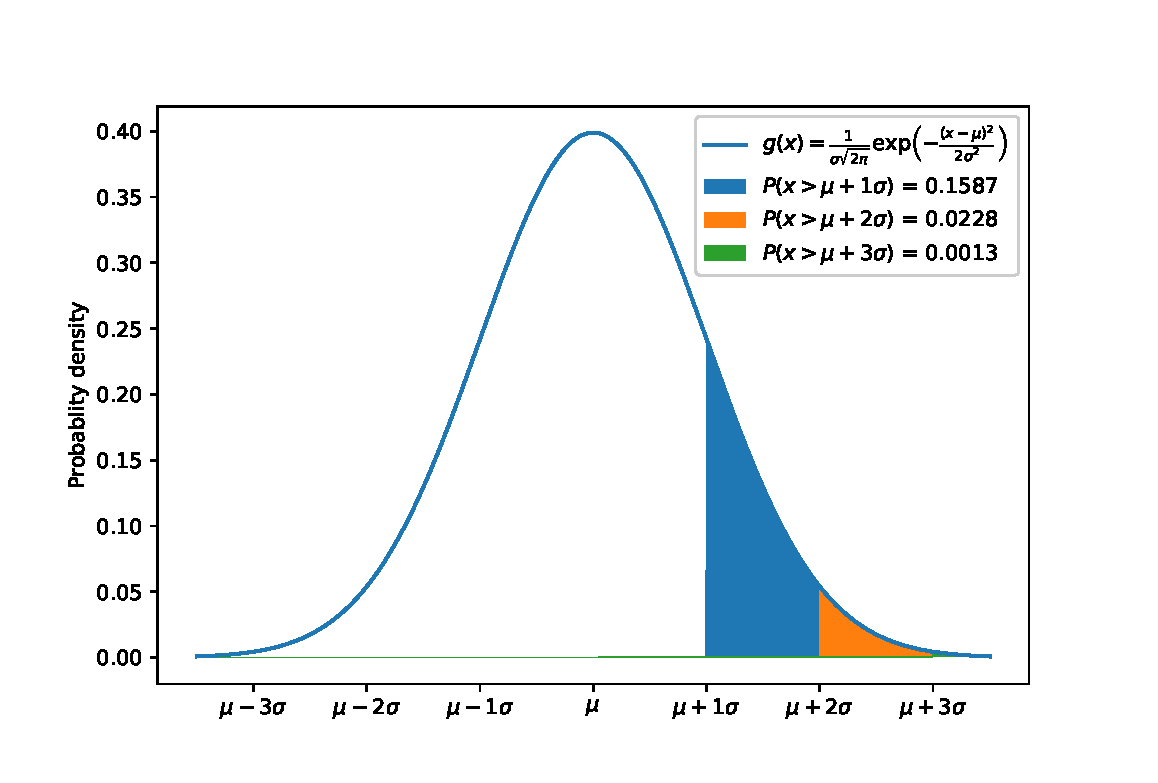
\includegraphics[width=9cm]{distribution}
\caption{Normal distribution and probability of having pixels with intensity above certain thresholds.}
\end{center}
\end{figure}

The storage space is much larger than just the pixel intensity since one needs to store as well also its position. 
Moreover, to be able to regenerate the background, the averaged and uncertainties curves needs to be stored.

The following section presents how the sparsification is performed on an example of Lysozyme dataset obtained using rotational data-collection.
Those data are then densified again to regenerate the data and processed in the standard XDS reduction tool \cite{xds}.
Data quality indicators are finally compared between the original dataset and the one which went through the lossy compression presented here.

\subsection{Sparsification}

The sigma-clipping algorithm was originally written for real-time sparsification of single crystal diffraction data and its integration into the LIMA2 \cite{lima} detector control system for the Jungfrau 4M detector used at ESRF ID29 is described in \cite{sri2021}.
The real-time constrain imposed to develop code running on GPU since those devices are several times
faster than equivalently priced processors.
All algorithms were developed in OpenCL \cite{opencl_khronos} and implemented in the \textit{pyFAI} software package.
A command line tool called `sparsify-Bragg' is available for off-line testing.

All the pixel coordinates and intensities are stored in a HDF5 container \cite{hdf5} following the nexus \cite{nexus} convention, together with a snippet of Python code explaining how to rebuild the dataset.
All sparse datasets (averaged and uncertainties curves, pixel coordinates, ...) are compressed with the bitshuffle-LZ4 \cite{bitshuffle} lossless compression.

\subsection{Densification}
Since no crystallographic software package is aware (yet) of this sparse format, the densification code was developed to regenerate initial frames and the `densify-Bragg` program was made available as part of the FabIO \cite{fabio} software package (version $\ge$0.12). 
The software constrains for this densification code are very different from the one for sparisfication since this code can be used by the final users.
For this reason `densify-Bragg' was optimized to run on multicore CPU.
The only important options are, beside the file-format and file-name, whether the background noise has to be reconstructed or not. 
Some crystallographic reduction program like CrysAlisPro \cite{crysalis} provide a better result without noisy background while XDS \cite{xds}, which performs a deep noise analysis, needs to have the noisy background restored. 
Shaded regions are never reconstructed properly and should be masked adequately in the reduction software.

\subsection{Performances}
The performances for a lossy compression algorithm are to be evaluated along many directions: compression and decompression speeds, compression ratio and degradation of the recorded signal.
All those factors have been evaluated on a classical sample, Lysozyme, and rotational data were collected on an Eiger 4M detector (selected for its similarity in size and performances with the Jungfrau detector). 
This reference dataset is the one made publicly available by Dectris TODO \cite{lysozyme}. 

\subsubsection{Compression ratio:} 
After sparsification (picking cut-off: $2\sigma$, error-model: Poisonnian), the dataset still weights 103MB which represents a 15x compression ratio compared to the standard procedure.
For conformance with the state of the art, the reference dataset was re-compressed using the bitshuffle-LZ4 algorithm \cite{bitshuffle}, for which the 1800 frames weight 1500MB (instead of the 5000GB of the original files compressed in LZ4).

The maximum theoretical compression ratio for $2\sigma$ is 22x (figure \ref{distribution}, neglecting the storage of the background data and effects of the lossless compression).
To evaluate the effective maximal compression ratio, the dataset was median-filtered along the image stack
to produce an image without peaks. 
A background dataset of 1800 such images sparsifies into a 11MB HDF5 file which represents a compression ratio of 136x ! 
Indeed, only 19 pixels were saved per frame and the compressed numerical values are mostly the same, which compresses great with bitshuffle-LZ4.

In production conditions, one would like to tune this threshold to the minimal value which guarantees a compression ratio large enough to allow the storage of all data.
For ESRF-ID29, where a Jungfrau 4M is operating at 1kHz, some `pedestal` preprocessing convert 16-bits integers into 32-bits floating point values and double the needed bandwidth for data saving. 
The detector outputs the data via 8x 10 Gbit/s network links and the storage is performed via  a single  25 Gbit/s link, making a minimum compression ratio of 6.4x which is equivalent to a cutoff at $1.4\sigma$ (Fig. \ref{distribution}).


\subsubsection{Compression speed:}
%\begin{verbatim}
%kieffer@scisoft14:~/Dectris/EIGER_X_4M_lyso/demo$ sparsify-Bragg ../collect_01_00001_master.h5 -p ../geometry.poni  --bins 500 --unit="r_mm" --cycle=5 --cutoff-clip=0  --noise=1 --profile -m ../mask.npy --cutoff-pick=2.0 --error-model=poisson -o sparse.h5
%INFO:pyFAI.method_registry:Degrading method from Method(dim=1, split='pseudo', algo='histogram', impl='*', target=None) -> Method(dim=1, split='bbox', algo='histogram', impl='*', target=None)
%INFO:pyFAI.geometry:Unable to parse ../geometry.poni as JSON file, defaulting to PoniParser
%WARNING:pyFAI.ext.splitBBoxCSR:Pixel splitting desactivated !
%INFO:silx.opencl.processing:379.313MB are needed on device: TITAN V,  which has 12652.839MB
%INFO:silx.opencl.processing:Compiling file ['silx:opencl/doubleword.cl', 'pyfai:openCL/preprocess.cl', 'pyfai:openCL/memset.cl', 'pyfai:openCL/ocl_azim_CSR.cl', 'pyfai:openCL/peak_finder.cl', 'pyfai:openCL/peakfinder8.cl'] with options -D NBINS=500  -D NIMAGE=4485690 -D WORKGROUP_SIZE=1024
%INFO:silx.opencl.processing:■■■■■■■■■■■■■■■■■■■]  100%  Saving: sparse.h5                      
%OpenCL kernel profiling statistics in milliseconds for: OCL_PeakFinder
%                                       Kernel name (count):      min   median      max     mean      std
%                                 copy H->D indices (    1):    3.730    3.730    3.730    3.730    0.000
%                                  copy H->D indptr (    1):    0.001    0.001    0.001    0.001    0.000
%                                    copy H->D mask (    1):    1.096    1.096    1.096    1.096    0.000
%                                copy H->D radius1d (    1):    0.002    0.002    0.002    0.002    0.000
%                                copy H->D radius2d (    1):    3.489    3.489    3.489    3.489    0.000
%                               copy raw H->D image ( 1800):    3.615    5.064    5.718    4.893    0.412
%                                 cast u32_to_float ( 1800):    0.070    0.075    0.103    0.074    0.001
%                                         memset_ng ( 1800):    0.004    0.004    0.010    0.004    0.000
%                                       corrections ( 1800):    0.169    0.171    0.178    0.172    0.001
%                                   csr_sigma_clip4 ( 1800):    3.077    3.230    4.140    3.267    0.133
%                                    memset counter ( 1800):    0.004    0.004    0.015    0.004    0.001
%                                       peak_search ( 1800):    0.261    0.263    0.272    0.263    0.001
%                                 copy D->H counter ( 1800):    0.001    0.001    0.010    0.001    0.000
%                  copy D->D + cast uint32 intenity ( 1800):    0.007    0.010    0.025    0.010    0.002
%                           copy D->H peak_position ( 1800):    0.003    0.006    0.029    0.009    0.005
%                           copy D->H peak_intensty ( 1800):    0.003    0.006    0.029    0.009    0.005
%                          copy D->H background_avg ( 1800):    0.002    0.002    0.004    0.002    0.000
%                          copy D->H background_std ( 1800):    0.002    0.002    0.003    0.002    0.000
%________________________________________________________________________________
%                       Total OpenCL execution time        : 15687.401ms
%\end{verbatim}

The compression speed has been measured on the computer designed for online data-reduction of the Jungfrau detector \cite{sri2021}: 
an IBM AC922 using two Power9 processors and two (to four) Nvidia Tesla V100 GPU. 
The sequential execution of the code on the GPU takes about 4 ms to process a one image and uses a single CPU-core and a quarter of a GPU. 
In online condition, multiple parallel processes are expected to achieve much higher frame-rate, since the nominal speed for the Jungfrau is 1kHz.

\subsubsection{Decompression speed:} 
The decompression of those data should typically be performed on a standard workstation (here running two Intel Xeon Gold 6134 CPU @ 3.20GHz): the reconstruction speed is found to take 30s while the writing of the densified dataset (with bitshuffle-LZ4 compression) takes 45s. 
%maybe explicit that the decompression is for the full dataset and not 30s per frame
Densification is thus faster than writing on disk.
The reading of the input sparse dataset is negligible (<2s).

\subsubsection{Quality of the restored dataset:} 
The densified dataset was processed via XDS and the summary indicator for the quality of the results are compared with the one coming from the reduction of the original dataset. 
Since those integrator are measured on integral peaks with $I/\sigma>3$ and the sparsification was performed
with a cut-off of 2, those result should be almost unaffected, which is confirmed in the table \ref{xds_summary}, hereafter.

\begin{table}[h]
\begin{center}
\label{xds_summary}
\caption{Quality indicators after peak integration and averaging using XDS\cite{xds}}.
\begin{tabular}{|c|c c c|c c c|} 
\hline
Indicator & \multicolumn{3}{c|}{Initial dataset} & \multicolumn{3}{c|}{Lossy compressed dataset ($2\sigma$)} \\ 
          & 2.91\AA & 2.06\AA & all & 2.91\AA & 2.06\AA & all \\
\hline
Completeness                                        & 98.8& 90.8 & 93.8\% & 99.8& 90.6 & 93.5\% \\ 
$R_{obs}=\frac{\sum |I_{h,i}-I_{i}|}{\sum I_{h,i}}$ & 9.9 & 57.3& 12.5\% & 9.2 & 61.2&  11.4\%\\ 
$R_{expected}$                                      & 8.8 & 73.2& 15.0\% & 8.2 & 68.7 &  12.1\%\\
$R_{meas}$ \cite{Rmeas}  &10.3 &61.2& 13.2\% & 9.6 & 65.5 & 12.0\%\\
$CC_{1/2}$ \cite{cc1/2}  & 99.7 &94.0 & 99.7   & 99.6 & 95.4 & 99.7  \\
$<I/\sigma>$               & 25.80 & 5.39 & 10.52  & 26.33& 4.09 & 10.17 \\
\hline
\end{tabular}
\end{center}
\end{table}


\section{Application to serial crystallography}
A classical way of pre-processing serial-crystallography data is to shrink the amount of data by sieving out empty frames, actually keeping frame which deserve to be saved ("Veto" algorithm).

The sigma clipping algorithm provides us with the background (average and deviation) and is used to pick pixels which are likely to be peaks. 
For this,  several additional checks are performed on the local neighborhood which is a small patch (typically 3x3 or 5x5 pixels):
\begin{itemize}
\item The considered pixel is the maximum of the local neighborhood.
\item The number of pixels in the local neighborhood satisfying the intensity condition ($|I-\bar{I} |> n \sigma_{I}$)  is above a given minimum.
\end{itemize}

For each peak, the pixel coordinate, the precise centroïd, the sum of the data and its propagated deviation are recorded and reported. 
Those results can be subsequently injected into CrystFEL \cite{CrystFEL} which is performing the indexing of
the data and validating if those peaks corresponds to an realistic crystal lattice \cite{nanopeakcell}.


\subsection{Quality of the extracted peaks}
Figure \ref{peakfinder} presents the comparison between the original "peakfinder8" described in \citeasnoun{Cheetah2014}, interfaced in Python via OnDA \cite{onda} and the version implemented into pyFAI. 

\begin{figure}
\label{peakfinder}
\begin{center}
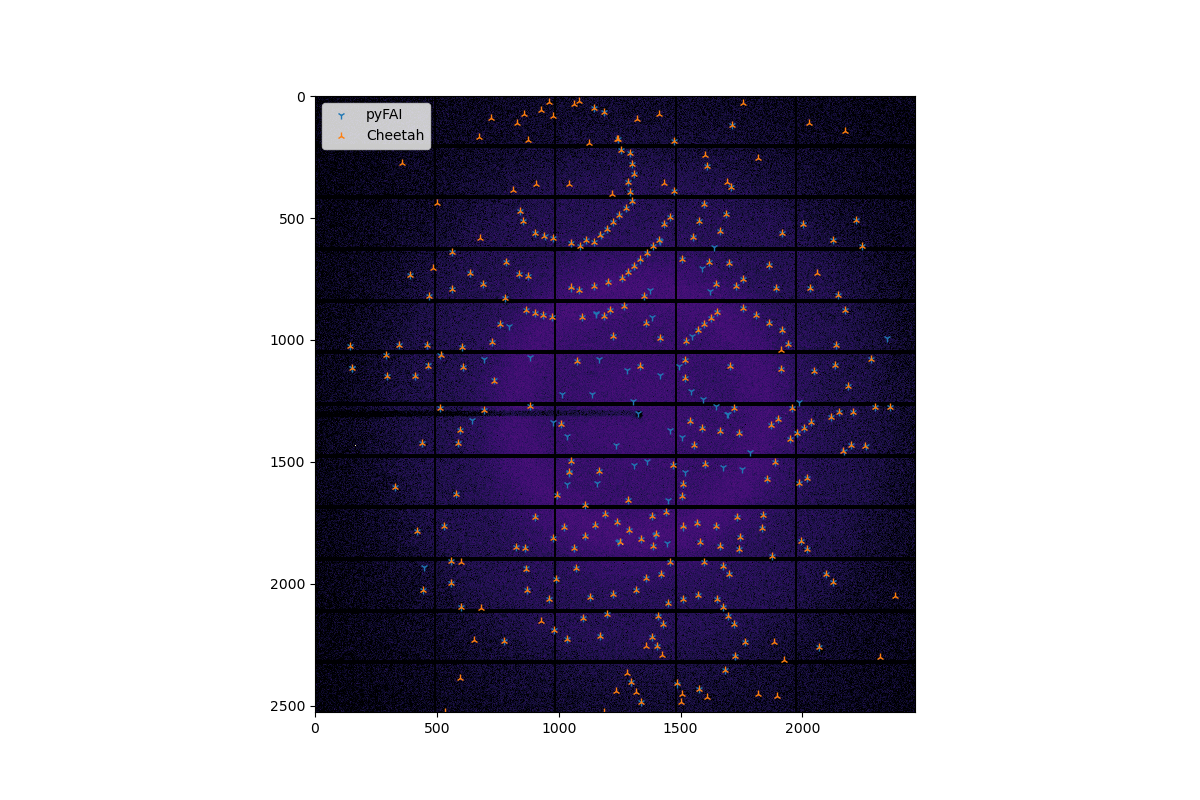
\includegraphics[width=12cm]{peakfinder}
\caption{Comparison of the reference \textit{peakfinder8} as implemented in Cheetah (in orange, execution time 300ms) and the version from pyFAI (in light blue, execution time 10ms) on top of a Pilatus6M MX diffraction frame.}
\end{center}
\end{figure}

TODO: analysis of those images 

TODO: indexing ratio in Crystfel

%JK: I am probably not using properly peakfinder8 ... any help welcome on that
\subsection{Performances}
The runtime fro pyFAI is 10ms while it takes 300ms for Cheetah ... but pyFAI performs has the calculation performed by a GPU which may not be generally available.
%Nota: The sigma-clipping is now available on CPU in pyFAI, but neither the compression nor the peakfinder is ported yet.

\section{Conclusion}

TODO:
Limitations: textured background


     %-------------------------------------------------------------------------
     % The back matter of the paper - acknowledgements and references
     %-------------------------------------------------------------------------

     % Acknowledgements come after the appendices

%\ack{Acknowledgements}
The authors would like to thank Gavin Vaughan, scientist at Materials beamline at the ESRF,  for the constructive discussion about sigma-clipping versus median filtering. 
We would like to thank also Jonathan P. Wright and Carlotta Giacobbe for offering us the ability to test those algorithms on small molecule data and validate the concept on the ID11 beamline from the ESRF.


\bibliographystyle{unsrt}
\bibliography{biblio}

\end{document}                    % DO NOT DELETE THIS LINE
%%%%%%%%%%%%%%%%%%%%%%%%%%%%%%%%%%%%%%%%%%%%%%%%%%%%%%%%%%%%%%%%%%%%%%%%%%%%%%
